\pdfbookmark{Общая характеристика работы}{characteristic}             % Закладка pdf
\section*{Общая характеристика работы}

\newcommand{\actuality}{\pdfbookmark[1]{Актуальность}{actuality}\textbf{\actualityTXT}}
\newcommand{\progress}{\pdfbookmark[1]{Разработанность темы}{progress}\textbf{\progressTXT}}
\newcommand{\aim}{\pdfbookmark[1]{Цели}{aim}{\textbf\aimTXT}}
\newcommand{\tasks}{\pdfbookmark[1]{Задачи}{tasks}\textbf{\tasksTXT}}
\newcommand{\aimtasks}{\pdfbookmark[1]{Цели и задачи}{aimtasks}\aimtasksTXT}
\newcommand{\novelty}{\pdfbookmark[1]{Научная новизна}{novelty}\textbf{\noveltyTXT}}
\newcommand{\influence}{\pdfbookmark[1]{Практическая значимость}{influence}\textbf{\influenceTXT}}
\newcommand{\methods}{\pdfbookmark[1]{Методология и методы исследования}{methods}\textbf{\methodsTXT}}
\newcommand{\defpositions}{\pdfbookmark[1]{Положения, выносимые на защиту}{defpositions}\textbf{\defpositionsTXT}}
\newcommand{\reliability}{\pdfbookmark[1]{Достоверность}{reliability}\textbf{\reliabilityTXT}}
\newcommand{\probation}{\pdfbookmark[1]{Апробация}{probation}\textbf{\probationTXT}}
\newcommand{\contribution}{\pdfbookmark[1]{Личный вклад}{contribution}\textbf{\contributionTXT}}
\newcommand{\publications}{\pdfbookmark[1]{Публикации}{publications}\textbf{\publicationsTXT}}


В диссертационной работе изучаются периодические режимы систем осцилляторов, функционирование каждого из которых описывается уравнением Мэки--Гласса. Для исследования релаксационных колебаний одиночного осциллятора используется метод малого параметра. Исследование периодических режимов проводится для систем осцилляторов релейного типа. %TODO: закончить мысль

{\actuality} Уравнениями Мэки--Гласса называют две модели с запаздыванием \cite{Mackey1977, Glass1988}:
\begin{equation}
	\label{eq:mg_equation_1:intro}
	\dot{u} = -\gamma u + \beta \dfrac{\theta^n u(t - \tau)}{\theta^n + u^n(t - \tau)},
\end{equation}
\begin{equation}
	\label{eq:mg_equation_2:intro}
	\dot{u} = -\gamma u + \beta \dfrac{\theta^n }{\theta^n + u^n(t - \tau)}.
\end{equation}

Данные модели были предложены для описания регуляторной функции в процессах кроветворения: здесь $u(t)$ имеет смысл концентрации кровяных телец, а запаздывание $\tau$ означает разницу во времени между сигналом к запуску процессов кроветворения и выпуском взрослых кровяных телец в кровь. Уравнения \eqref{eq:mg_equation_1:intro} и \eqref{eq:mg_equation_2:intro} отличаются функцией обратной связи: в уравнении \eqref{eq:mg_equation_2:intro} эта функция монотонно убывает, а в уравнении \eqref{eq:mg_equation_1:intro} имеет форму <<горба>> (\emph{hump function}). В данной работе под уравнением Мэки--Гласса будет пониматься уравнение \eqref{eq:mg_equation_1:intro}.

Уравнение Мэки--Гласса исследовалось во множестве работ \cite{Junges2012, Berezansky2006, Su2011, Liz2002, Wu2007, Kubyshkin2016}. Так, в оригинальном исследовании \cite{Mackey1977} приводятся численные решения как в форме периодических, так и непериодических колебаний. В работах \cite{Berezansky2006, Liz2002} исследуются условия, при которых решение уравнения отделено от нуля (англ. \emph{persistence}), либо стремится к нулю при $t \to +\infty$ (англ. \emph{extinction}). В \cite{Berezansky2006, Kubyshkin2016} проводится анализ устойчивости постоянного решения $v \equiv  \theta \left(\frac{a}{b} - 1\right)^{1/\gamma}$. Также в \cite{Kubyshkin2016} исследуются решения, бифурцирующие из постоянного решения. 

Уравнение Мэки--Гласса и различные его модификации широко использовалось при моделировании функционирования электрогенераторов \cite{Tateno2012, Namajunas1995, Glyzin2018, Glyzin2018a}, а также для симуляции хаотического сигнала \cite{Grassberger1983, Amil2015, Amil2015a, Shahverdiev2006}. В работах \cite{Bartha2021, Krisztin2020} изучаются периодические решения уравнения Мэки--Гласса, в частности, в работе \cite{Bartha2021} при некоторых ограничениях на параметры доказывается существование и единственность предельного цикла, который является экспоненциально орбитально устойчивым.

Интерес представляет исследование систем, отвечающих цепям генераторов Мэки--Гласса \cite{Preobrazhenskaia2021, Tateno2012, Sano2007, Wan2009}. В статье \cite{Sano2007} численно и экспериментально изучалась система из четырех генераторов Мэки--Гласса, два из которых были вещательными, а два --- принимающими. Система обладала петлей обратной связи. В работе приведена подробная схема электрической цепи, а также описан эксперимент, в результате которого установлена двойная синхронизация хаотического сигнала. В работе \cite{Wan2009} для той же системы исследовалась колебательная потеря устойчивости состояния равновесия.

Подобная система генераторов Мэки--Гласса, но для двух уравнений и с несколько иным способом связи, рассматривалась в работе \cite{Tateno2012}. В исследуемой цепи генераторы также были двух типов: один вещатель и одно принимающее устройство. В модели было две петли обратной связи с запаздыванием по времени. Для нее экспериментально и численно исследовалась генерация хаоса. Показано, что соотношение двух запаздываний имеет решающую роль для усиления или подавления хаотической динамики. Также в данной работе показано, что качественная синхронизация хаоса может быть достигнута при высокой силе связи и условиях согласования параметров между двумя электронными схемами.

Пусть в распоряжении имеется произвольное (фиксированное) число генераторов. Выделим две естественные структуры для связи генераторов: кольцо (рис. \ref{fig:ring:intro}) и полносвязная цепь, где каждый связан с каждым (рис. \ref{fig:full_mesh:intro}). В том и другом случае можно поставить вопрос о поиске дискретных бегущих волн --- таких решений, что все компоненты представлены одной и той же функцией с кратными сдвигами (строгое описание таких решений будет приведено в следующем пункте). Методика поиска бегущих волн и доказательства устойчивости в кольцевых цепях описана в работе \cite{Glyzin2012}, а для полносвязной цепи --- в \cite{Глызин2022}.

\begin{figure}[ht]
	\begin{minipage}[b]{0.45\linewidth}
		\centering
		\includegraphics[width=\textwidth]{mg_generator_ring.eps}
		\caption{Кольцо генераторов. Каждый генератор является принимающим для предыдущего, и передающим для следующего в кольце генератора.}
		\label{fig:ring:intro}
	\end{minipage}
	\hspace{0.5cm}
	\begin{minipage}[b]{0.45\linewidth}
		\centering
		\includegraphics[width=\textwidth]{mg_generator_full.eps}
		\caption{Полносвязная цепь генераторов. Каждый генератор является передающим и принимающим для всех остальных генераторов в цепи.}
		\label{fig:full_mesh:intro}
	\end{minipage}
\end{figure}



Обзор, введение в тему, обозначение места данной работы в
мировых исследованиях и~т.\:п., можно использовать ссылки на~другие
работы~(если их~нет, то~в~автореферате
автоматически пропадёт раздел <<Список литературы>>). Внимание! Ссылки
на~другие работы в~разделе общей характеристики работы можно
использовать только при использовании \verb!biblatex! (из-за технических
ограничений \verb!bibtex8!. Это связано с тем, что одна
и~та~же~характеристика используются и~в~тексте диссертации, и в
автореферате. В~последнем, согласно ГОСТ, должен присутствовать список
работ автора по~теме диссертации, а~\verb!bibtex8! не~умеет выводить в~одном
файле два списка литературы).
При использовании \verb!biblatex! возможно использование исключительно
в~автореферате подстрочных ссылок
для других работ командой \verb!\autocite!, а~также цитирование
собственных работ командой \verb!\cite!. Для этого в~файле
\verb!common/setup.tex! необходимо присвоить положительное значение
счётчику \verb!\setcounter{usefootcite}{1}!.

Для генерации содержимого титульного листа автореферата, диссертации
и~презентации используются данные из файла \verb!common/data.tex!. Если,
например, вы меняете название диссертации, то оно автоматически
появится в~итоговых файлах после очередного запуска \LaTeX. Согласно
ГОСТ 7.0.11-2011 <<5.1.1 Титульный лист является первой страницей
диссертации, служит источником информации, необходимой для обработки и
поиска документа>>. Наличие логотипа организации на~титульном листе
упрощает обработку и~поиск, для этого разметите логотип вашей
организации в папке images в~формате PDF (лучше найти его в векторном
варианте, чтобы он хорошо смотрелся при печати) под именем
\verb!logo.pdf!. Настроить размер изображения с логотипом можно
в~соответствующих местах файлов \verb!title.tex!  отдельно для
диссертации и автореферата. Если вам логотип не~нужен, то просто
удалите файл с~логотипом.

\ifsynopsis
Этот абзац появляется только в~автореферате.
Для формирования блоков, которые будут обрабатываться только в~автореферате,
заведена проверка условия \verb!\!\verb!ifsynopsis!.
Значение условия задаётся в~основном файле документа (\verb!synopsis.tex! для
автореферата).
\else
Этот абзац появляется только в~диссертации.
Через проверку условия \verb!\!\verb!ifsynopsis!, задаваемого в~основном файле
документа (\verb!dissertation.tex! для диссертации), можно сделать новую
команду, обеспечивающую появление цитаты в~диссертации, но~не~в~автореферате.
\fi

% {\progress}
% Этот раздел должен быть отдельным структурным элементом по
% ГОСТ, но он, как правило, включается в описание актуальности
% темы. Нужен он отдельным структурынм элемементом или нет ---
% смотрите другие диссертации вашего совета, скорее всего не нужен.

{\aim} данной работы является \ldots

Для~достижения поставленной цели необходимо было решить следующие {\tasks}:
\begin{enumerate}[beginpenalty=10000] % https://tex.stackexchange.com/a/476052/104425
  \item Исследовать, разработать, вычислить и~т.\:д. и~т.\:п.
  \item Исследовать, разработать, вычислить и~т.\:д. и~т.\:п.
  \item Исследовать, разработать, вычислить и~т.\:д. и~т.\:п.
  \item Исследовать, разработать, вычислить и~т.\:д. и~т.\:п.
\end{enumerate}


{\novelty}
\begin{enumerate}[beginpenalty=10000] % https://tex.stackexchange.com/a/476052/104425
  \item Впервые \ldots
  \item Впервые \ldots
  \item Было выполнено оригинальное исследование \ldots
\end{enumerate}

{\influence} \ldots

{\methods} \ldots

{\defpositions}
\begin{enumerate}[beginpenalty=10000] % https://tex.stackexchange.com/a/476052/104425
  \item Первое положение
  \item Второе положение
  \item Третье положение
  \item Четвертое положение
\end{enumerate}
В папке Documents можно ознакомиться с решением совета из Томского~ГУ
(в~файле \verb+Def_positions.pdf+), где обоснованно даются рекомендации
по~формулировкам защищаемых положений.

{\reliability} полученных результатов обеспечивается \ldots \ Результаты находятся в соответствии с результатами, полученными другими авторами.


{\probation}
Основные результаты работы докладывались~на:
перечисление основных конференций, симпозиумов и~т.\:п.

{\contribution} Автор принимал активное участие \ldots

\ifnumequal{\value{bibliosel}}{0}
{%%% Встроенная реализация с загрузкой файла через движок bibtex8. (При желании, внутри можно использовать обычные ссылки, наподобие `\cite{vakbib1,vakbib2}`).
    {\publications} Основные результаты по теме диссертации изложены
    в~XX~печатных изданиях,
    X из которых изданы в журналах, рекомендованных ВАК,
    X "--- в тезисах докладов.
}%
{%%% Реализация пакетом biblatex через движок biber
    \begin{refsection}[bl-author, bl-registered]
        % Это refsection=1.
        % Процитированные здесь работы:
        %  * подсчитываются, для автоматического составления фразы "Основные результаты ..."
        %  * попадают в авторскую библиографию, при usefootcite==0 и стиле `\insertbiblioauthor` или `\insertbiblioauthorgrouped`
        %  * нумеруются там в зависимости от порядка команд `\printbibliography` в этом разделе.
        %  * при использовании `\insertbiblioauthorgrouped`, порядок команд `\printbibliography` в нём должен быть тем же (см. biblio/biblatex.tex)
        %
        % Невидимый библиографический список для подсчёта количества публикаций:
        \printbibliography[heading=nobibheading, section=1, env=countauthorvak,          keyword=biblioauthorvak]%
        \printbibliography[heading=nobibheading, section=1, env=countauthorwos,          keyword=biblioauthorwos]%
        \printbibliography[heading=nobibheading, section=1, env=countauthorscopus,       keyword=biblioauthorscopus]%
        \printbibliography[heading=nobibheading, section=1, env=countauthorconf,         keyword=biblioauthorconf]%
        \printbibliography[heading=nobibheading, section=1, env=countauthorother,        keyword=biblioauthorother]%
        \printbibliography[heading=nobibheading, section=1, env=countregistered,         keyword=biblioregistered]%
        \printbibliography[heading=nobibheading, section=1, env=countauthorpatent,       keyword=biblioauthorpatent]%
        \printbibliography[heading=nobibheading, section=1, env=countauthorprogram,      keyword=biblioauthorprogram]%
        \printbibliography[heading=nobibheading, section=1, env=countauthor,             keyword=biblioauthor]%
        \printbibliography[heading=nobibheading, section=1, env=countauthorvakscopuswos, filter=vakscopuswos]%
        \printbibliography[heading=nobibheading, section=1, env=countauthorscopuswos,    filter=scopuswos]%
        %
        \nocite{*}%
        %
        {\publications} Основные результаты по теме диссертации изложены в~\arabic{citeauthor}~печатных изданиях,
        \arabic{citeauthorvak} из которых изданы в журналах, рекомендованных ВАК\sloppy%
        \ifnum \value{citeauthorscopuswos}>0%
            , \arabic{citeauthorscopuswos} "--- в~периодических научных журналах, индексируемых Web of~Science и Scopus\sloppy%
        \fi%
        \ifnum \value{citeauthorconf}>0%
            , \arabic{citeauthorconf} "--- в~тезисах докладов.
        \else%
            .
        \fi%
        \ifnum \value{citeregistered}=1%
            \ifnum \value{citeauthorpatent}=1%
                Зарегистрирован \arabic{citeauthorpatent} патент.
            \fi%
            \ifnum \value{citeauthorprogram}=1%
                Зарегистрирована \arabic{citeauthorprogram} программа для ЭВМ.
            \fi%
        \fi%
        \ifnum \value{citeregistered}>1%
            Зарегистрированы\ %
            \ifnum \value{citeauthorpatent}>0%
            \formbytotal{citeauthorpatent}{патент}{}{а}{}\sloppy%
            \ifnum \value{citeauthorprogram}=0 . \else \ и~\fi%
            \fi%
            \ifnum \value{citeauthorprogram}>0%
            \formbytotal{citeauthorprogram}{программ}{а}{ы}{} для ЭВМ.
            \fi%
        \fi%
        % К публикациям, в которых излагаются основные научные результаты диссертации на соискание учёной
        % степени, в рецензируемых изданиях приравниваются патенты на изобретения, патенты (свидетельства) на
        % полезную модель, патенты на промышленный образец, патенты на селекционные достижения, свидетельства
        % на программу для электронных вычислительных машин, базу данных, топологию интегральных микросхем,
        % зарегистрированные в установленном порядке.(в ред. Постановления Правительства РФ от 21.04.2016 N 335)
    \end{refsection}%
    \begin{refsection}[bl-author, bl-registered]
        % Это refsection=2.
        % Процитированные здесь работы:
        %  * попадают в авторскую библиографию, при usefootcite==0 и стиле `\insertbiblioauthorimportant`.
        %  * ни на что не влияют в противном случае
        \nocite{vakbib2}%vak
        \nocite{patbib1}%patent
        \nocite{progbib1}%program
        \nocite{bib1}%other
        \nocite{confbib1}%conf
    \end{refsection}%
        %
        % Всё, что вне этих двух refsection, это refsection=0,
        %  * для диссертации - это нормальные ссылки, попадающие в обычную библиографию
        %  * для автореферата:
        %     * при usefootcite==0, ссылка корректно сработает только для источника из `external.bib`. Для своих работ --- напечатает "[0]" (и даже Warning не вылезет).
        %     * при usefootcite==1, ссылка сработает нормально. В авторской библиографии будут только процитированные в refsection=0 работы.
}

При использовании пакета \verb!biblatex! будут подсчитаны все работы, добавленные
в файл \verb!biblio/author.bib!. Для правильного подсчёта работ в~различных
системах цитирования требуется использовать поля:
\begin{itemize}
        \item \texttt{authorvak} если публикация индексирована ВАК,
        \item \texttt{authorscopus} если публикация индексирована Scopus,
        \item \texttt{authorwos} если публикация индексирована Web of Science,
        \item \texttt{authorconf} для докладов конференций,
        \item \texttt{authorpatent} для патентов,
        \item \texttt{authorprogram} для зарегистрированных программ для ЭВМ,
        \item \texttt{authorother} для других публикаций.
\end{itemize}
Для подсчёта используются счётчики:
\begin{itemize}
        \item \texttt{citeauthorvak} для работ, индексируемых ВАК,
        \item \texttt{citeauthorscopus} для работ, индексируемых Scopus,
        \item \texttt{citeauthorwos} для работ, индексируемых Web of Science,
        \item \texttt{citeauthorvakscopuswos} для работ, индексируемых одной из трёх баз,
        \item \texttt{citeauthorscopuswos} для работ, индексируемых Scopus или Web of~Science,
        \item \texttt{citeauthorconf} для докладов на конференциях,
        \item \texttt{citeauthorother} для остальных работ,
        \item \texttt{citeauthorpatent} для патентов,
        \item \texttt{citeauthorprogram} для зарегистрированных программ для ЭВМ,
        \item \texttt{citeauthor} для суммарного количества работ.
\end{itemize}
% Счётчик \texttt{citeexternal} используется для подсчёта процитированных публикаций;
% \texttt{citeregistered} "--- для подсчёта суммарного количества патентов и программ для ЭВМ.

Для добавления в список публикаций автора работ, которые не были процитированы в
автореферате, требуется их~перечислить с использованием команды \verb!\nocite! в
\verb!Synopsis/content.tex!.
 % Характеристика работы по структуре во введении и в автореферате не отличается (ГОСТ Р 7.0.11, пункты 5.3.1 и 9.2.1), потому её загружаем из одного и того же внешнего файла, предварительно задав форму выделения некоторым параметрам

%Диссертационная работа была выполнена при поддержке грантов \dots

%\underline{\textbf{Объем и структура работы.}} Диссертация состоит из~введения,
%четырех глав, заключения и~приложения. Полный объем диссертации
%\textbf{ХХХ}~страниц текста с~\textbf{ХХ}~рисунками и~5~таблицами. Список
%литературы содержит \textbf{ХХX}~наименование.

\pdfbookmark{Содержание работы}{description}                          % Закладка pdf
\section*{Содержание работы}

\pdfbookmark{Содержание первой главы}{chfirst}
\paragraph{Содержание первой главы.} В первой главе исследуется уравнение Мэки--Гласса в предположении, что показатель степени в знаменателе нелинейности --- большой параметр. Рассматривается случай, в котором релейное уравнение, возникающее при устремлении большого параметра к бесконечности, имеет периодическое решение с наименьшим числом переключений релейной части на периоде. Для данного случая доказывается существование периодического решения уравнения Мэки--Гласса, асимптотически близкого периодическому решению предельного уравнения.

Уравнение Мэки--Гласса \eqref{eq:mg_equation_1:intro} после нормировки параметров и времени принимает вид
\begin{equation}
	\label{eq:intro:mg_norm}
	\dot{u}=-\beta u+\frac{\alpha u(t-1)}{1+(u(t-1))^\gamma}, \text{ где } \alpha > 0, \beta > 0, \gamma > 0.
\end{equation}

Для положительных начальных функций решение уравнения \eqref{eq:intro:mg_norm} также положительно, поэтому корректна замена $u = e^x$, после которой это уравнение примет вид
\begin{equation}
	\label{eq:intro:MG_x}
	\dot{x}=-\beta+\alpha\frac{e^{x(t-1)-x}}{1+e^{\gamma x(t-1)}}.
\end{equation}

Будем считать $\gamma$ большим параметром. При $\gamma \to +\infty$ получаем релейное уравнение
\begin{equation}
	\label{eq:intro:MG_rele}
	\dot{x}=-\beta + \alpha e^{-x} F(\exp({x(t-1)})),
\end{equation}
где
\begin{equation}
	\label{eq:intro:F}
	F(u)=\lim\limits_{\gamma\to +\infty}\frac{u}{1+u^{\gamma}}=
	\begin{cases}
		0, & u > 1,\\
		\frac{1}{2}, & u = 1,\\
		u, & 0 \leq u < 1.
	\end{cases}
\end{equation}

Определим множество начальных функций, для которых затем явно будет построено решение предельного уравнения методом шагов. Зафиксируем положительные параметры $\sigma_0 < 1/2$, $p$, $q$ такие, что 
%
\[0 < p < \beta \sigma_0 < q.\]
%
В качестве множества начальных функций для уравнений \eqref{eq:intro:MG_x} и \eqref{eq:intro:MG_rele} зададим множество
\begin{multline}
	\label{eq:intro:init_set}
	S=\{\varphi\in C[-1 - \sigma_0, -\sigma_0]: 0 < p \leqslant \varphi(t)\leqslant q \text{ при } t \in [-1 - \sigma_0, -\sigma_0],\\ \varphi(-\sigma_0) = \beta \sigma_0 \}.
\end{multline}

\begin{figure}
	\centering
	\includegraphics[width=0.7\textwidth]{initial_func_S.eps}
	\caption{Представитель множества \eqref{eq:intro:init_set} начальных функций уравнений \eqref{eq:intro:MG_x} и \eqref{eq:intro:MG_rele}.}
	\label{fig:intro:initial_funcs:ch1}
\end{figure}

Введём обозначения:
\begin{equation}
	\label{eq:intro:T}
	T = \frac{1}{\beta} \ln\left(\frac{1}{2}\alpha^2e^{2\beta}(t_1 - 2)^2 + \alpha e^{\beta}(t_1 - 1) + 1\right),
\end{equation}
где $t = t_1$ --- корень уравнения 
\begin{equation}
	\label{eq:intro:t1_cond_exp}
	-\beta(t - 1) + \ln(\alpha e^{\beta}(t - 2) + 1) = 0,
\end{equation}
\begin{equation}
	\label{eq:intro:t2_period}
	t_2 = 1 + T.
\end{equation}

Доказано следующее утверждение.

\textbf{Теорема} (О решении релейного уравнения). \textit{
	Пусть параметры $\alpha, \beta > 0$ удовлетворяют условиям
	%
	\begin{equation}
		\label{eq:intro:cond_alpha1}
		\begin{cases}
			\left[
			\begin{array}{ll}
				\alpha > e^{\beta} - e^{-\beta},\\
				\alpha < \beta e^{\beta},
			\end{array}
			\right.\\
			\frac{\alpha}{\beta}e^{\beta}\left(1 + \ln\frac{\beta}{\alpha}\right) < 1,
		\end{cases}
	\end{equation}
	\begin{equation}
		\label{eq:intro:cond_alpha2}
		\alpha > \dfrac{e^{\beta t_1} - 1}{e^{\beta}(t_1 - 1)}.
	\end{equation}
	%
	Тогда уравнение \eqref{eq:intro:MG_rele} с начальной функцией из множества \eqref{eq:intro:init_set} имеет $T$-периодическое решение
	\small
	\begin{equation}
		\label{eq:intro:sol_x_star}
		x^*(t)= 
		\begin{cases}
			-\beta t, & t\in[-\sigma_0, 1],\\
			-\beta t +\ln(\alpha e^{\beta}(t - 1)+1), & t\in[1, 2],\\
			-\beta t + \ln(\frac{\alpha^2}{2}e^{2\beta}(t - 2)^2+\alpha e^{\beta}(t - 1)+1), & t\in[2, t_1],\\
			-\beta t + \ln(\frac{\alpha^2}{2}e^{2\beta}(t_1 - 2)^2+\alpha e^{\beta}(t_1 - 1) + 1), & t\in[t_1, t_2].
		\end{cases}
	\end{equation}
	\normalsize
}

Изображение цикла \eqref{eq:intro:sol_x_star} приведено на рисунке \ref{fig:intro:x_star:ch1}.

% 2024-01-21-mackey-glass-asymptotics.ipynb
\begin{figure}
	\centering
	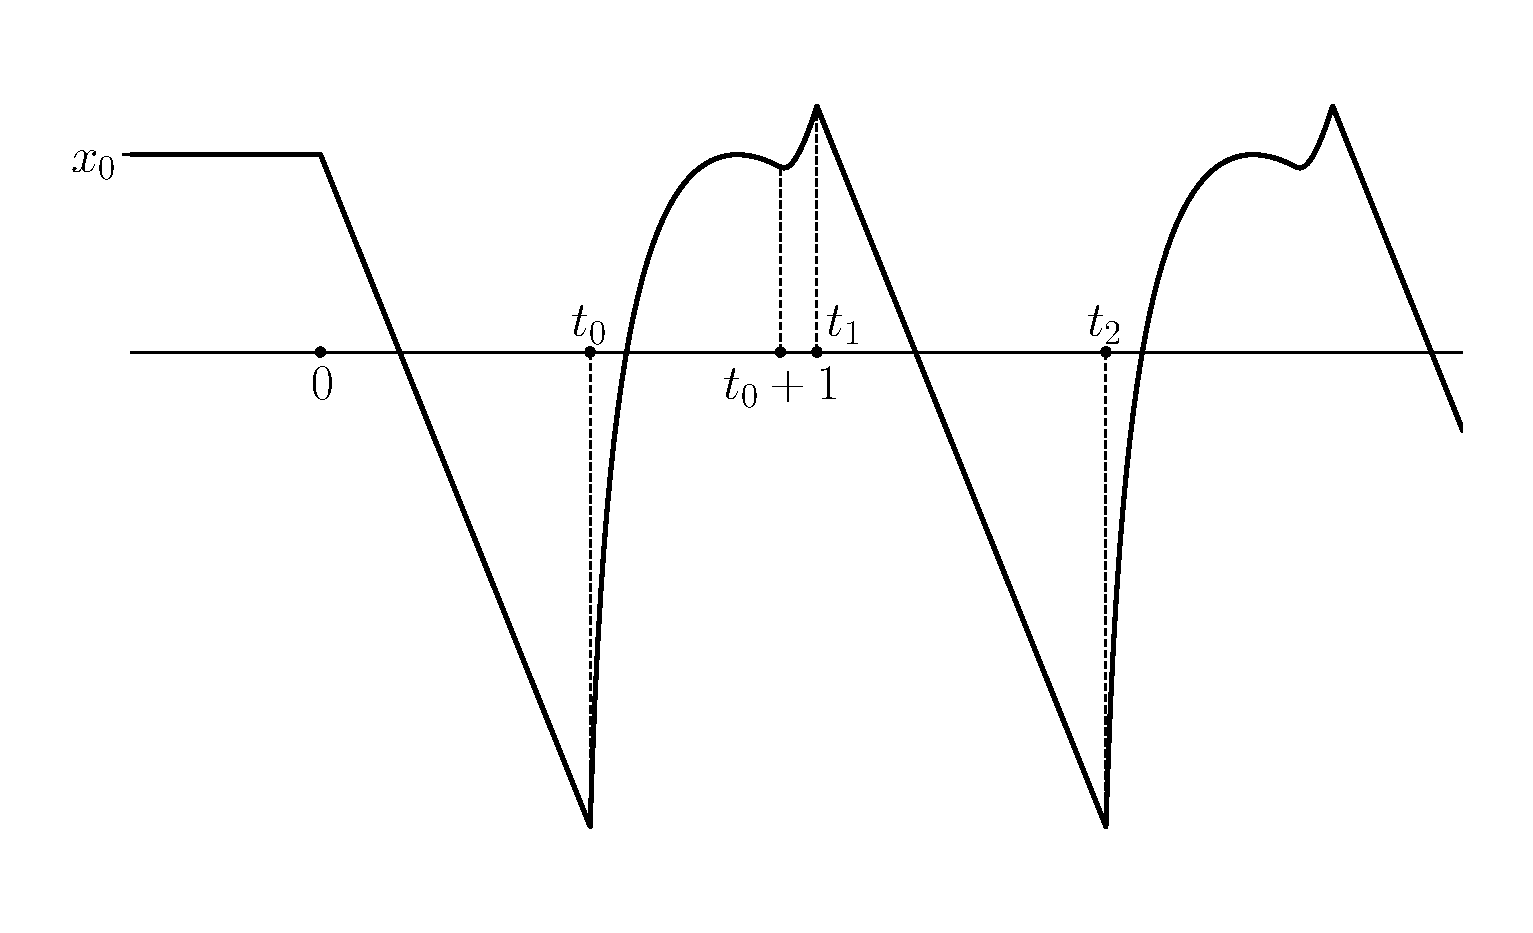
\includegraphics[width=0.7\textwidth]{x_star.eps}
	\captionof{figure}{Периодическое решение $x^{*}(t)$ уравнения \eqref{eq:intro:MG_rele}.}
	\label{fig:intro:x_star:ch1}
\end{figure}

Введём вспомогательные функции $w_i(\tau)$, $i = 0, 1$ для описания решения в окрестностях точек излома релейного уравнения.
\[
w_i(\tau) = -\beta \tau - \dfrac{\alpha e^{-x^*(t_i)}}{\dot{x}^*(t_i - 1)} \ln\left(e^{-\dot{x}^*(t_i - 1)\tau} + 1\right) \quad \text{при} \quad \dot{x}^*(t_i - 1) > 0,
\]
\[
w_i(\tau) = (-\beta + \alpha e^{-x^*(t_i)})\tau - \dfrac{\alpha e^{-x^*(t_i)}}{\dot{x}^*(t_i - 1)} \ln\left(e^{\dot{x}^*(t_i - 1)\tau} + 1\right) \quad \text{при} \quad \dot{x}^*(t_i - 1) < 0,
\]
Соответствующие значения функции $x^*(t)$ находится из формул \eqref{eq:intro:sol_x_star}.

Данные функции удовлетворяют асимптотическим свойствам.

Если $\dot{x}(t_i - 1) < 0$,
\begin{equation*}
	w_i(\tau) = -\beta \tau + O(\exp(-\dot{x}^*(t_i - 1) \tau)) \text{ при } \tau \to -\infty,
\end{equation*}
\begin{equation*}
	w_i(\tau) = (-\beta + \alpha e^{-x^*(t_i)})\tau + O(\exp(\dot{x}^*(t_i - 1) \tau)) \text{ при } \tau \to +\infty,
\end{equation*}

Если $\dot{x}(t_i - 1) > 0$,
\begin{equation*}
	w_i(\tau) = (-\beta + \alpha e^{-x^*(t_i)})\tau + O(\exp(\dot{x}^*(t_i - 1) \tau)) \text{ при } \tau \to -\infty,
\end{equation*}
\begin{equation*}
	w_i(\tau) = -\beta \tau + O(\exp(-\dot{x}^*(t_i - 1) \tau)) \text{ при } \tau \to +\infty.
\end{equation*}

Коэффициенты при $\tau$ в приведённых формулах совпадают с односторонними производными в точках излома решения релейного уравнения $t_i$ при $i = 0, 1$.

Основной результат главы формулируется следующим образом.

\bigskip

\textbf{Теорема.} \textit{Пусть параметры $\alpha > \beta > 0$ удовлетворяют условиям \eqref{eq:intro:cond_alpha1}, \eqref{eq:intro:cond_alpha2}. Тогда существуют такие значения параметров $\sigma_0, p, q$ и такое достаточно большое $\gamma_0$, что при всех $\gamma > \gamma_0$ уравнение \eqref{eq:intro:MG_x} с начальной функцией $\varphi$ из множества \eqref{eq:intro:init_set} обладает периодическим решением $x^*_\gamma(t, \varphi)$ периода $T_{\gamma, \varphi}$ с асимптотикой}
\footnotesize
\begin{equation}
	\label{eq:intro:sol_x*gamma}
	x^*_\gamma(t, \varphi)= 
	\begin{cases}
		- \beta t + O(\gamma^{-1} e^{-\beta \delta \gamma}), & t\in[-\sigma_0, 1 - \delta],\\
		-\beta + \frac{1}{\gamma} w_0(\tau)|_{\tau=(t - 1)\gamma} + O(\gamma^{-2\nu}), & t \in [1 - \delta,1 + \delta],\\
		- \beta t + \ln(\alpha e^{\beta}(t - 1) + 1) + O(\gamma^{-2\nu}) & t\in[1 + \delta, 2]\\
		- \beta t + \ln(\frac{\alpha^2}{2}e^{2 \beta}(t - 2)^2 + \alpha e^{\beta}(t - 1) + 1) + O(\gamma^{-2\nu}), & t \in [2, t_1 - \delta],\\
		- \beta t_1 + \ln(\eta)+\frac{1}{\gamma} w_1(\tau)|_{\tau=(t - t_1)\gamma} + O(\gamma^{-2\nu}), & t\in[t_1 - \delta, t_1  +\delta],\\
		- \beta t + \ln(\eta) + O(\gamma^{-2\nu}), & t \in [t_1 + \delta, t_2 - \delta],
	\end{cases}
\end{equation}
\normalsize
где $\nu \in (\frac{1}{2}, 1)$, $\delta = \gamma^{-\nu}$, $\eta=\frac{\alpha^2}{2}e^{2\beta}(t_1 - 2)^2 + \alpha e^{\beta}(t_1 - 1) + 1$.
%
\textit{Данное решение удовлетворяет предельным равенствам}
%
\begin{equation}
	\label{eq:intro:lim_x*}
	\lim_{\gamma\to+\infty}\max_{0\leqslant t\leqslant T_{\gamma, \varphi}}|x_{\gamma}^*(t, \phi)-x^*(t)|=0,\quad \lim_{\gamma\to+\infty}T_{\gamma, \varphi} = T.
\end{equation}
\textit{Все остатки и пределы равномерны по $\varphi \in S$ и $t$ из соответствующих промежутков.}

\pdfbookmark{Содержание второй главы}{chsecond}
\textbf{Содержание второй главы.} Во второй главе рассматривается полносвязная сеть релейных осцилляторов Мэки--Гласса, описываемая системой \eqref{eq:intro:mg_full_renormed}. Будем искать решение в виде дискретной бегущей волны. После подстановки $u_j(t) = u(t + j\Delta)$ получим вспомогательное уравнение \eqref{eq:intro:mg_auxiliary}.

Нормируем время так, чтобы наименьшее из запаздываний вспомогательного уравнения стало равно 1. Пусть $1 = \tau_0 \leq \tau_1 \leq \ldots \leq \tau_N$ --- множество запаздываний после нормировки. Получим уравнение 
\begin{equation}
	\label{eq:intro:mg_relay_w}
	\dot{u}=-\beta u+\alpha F(w(t)), \text{ где } w(t) = \sum\limits_{s = 0}^N u(t - \tau_s).
\end{equation}
%
Определим множество начальных функций на промежутке длины наибольшего запаздывания: 
%
\begin{equation}
	\label{eq:intro:mg_init_set}
	\{\varphi\in C[-\tau_{N},0]:\  \varphi(t)>1 \text{ при } t\in[-\tau_{N},0),\ \varphi(0)=u_0 > 1\}.
\end{equation}
%
Введём обозначения:
%
\begin{equation*}
	A = \sum_{i=0}^{m}e^{\beta \tau_{i}}=e^\beta+e^{\beta \tau_1}+\ldots+e^{\beta \tau_{N}},
\end{equation*}
\begin{equation*}
	\tau_* = \min\{2,\tau_1\}=\left\lbrace\begin{array}{cl}
		\min\{2,1/\Delta\}, & \text{ если } \Delta < 1,
		\\
		\min\{2,\Delta\}, & \text{ если } \Delta > 1,
	\end{array}\right.
\end{equation*}
\begin{equation*}
	s_* = t_1-t_0.
\end{equation*}
%
Для вспомогательного уравнения \eqref{eq:intro:mg_relay_w} доказана следующая теорема.

\textbf{Теорема.} \textit{Пусть параметры $\alpha, \beta$ и величина $\tau_*$ удовлетворяют ограничениям}

\begin{equation}
	\label{eq:intro:cond_thm1}
	\frac{\alpha}{\beta}e^{\beta}\left(\ln\left(\frac{\beta}{\alpha}\right)+1\right) < 1,
	\quad
	\alpha > \beta.
\end{equation}
%
\begin{equation}
	\label{eq:intro:cond_thm2}
	e^{\beta \tau_*}-1 \leqslant \alpha e^\beta(\tau_*-1)
	\quad\text{или}\quad
	0 < \frac{1}{\beta}\ln\frac{\alpha}{\beta}\leqslant\tau_*-1,
\end{equation}
%
\begin{equation}
	\label{eq:intro:cond_th_w>1_t_1+1}
	e^{-\beta s_*}(e^{-\beta}+\alpha s_*)>1
\end{equation}
%
\begin{equation}
	\label{eq:intro:cond_hair_hair_01}
	\frac{\alpha^2}{2}e^\beta(s_*-1)^2+\alpha s_*>\frac{e^{\beta \tau_k}-1}{\sum_{i=0}^{k-1}e^{\beta \tau_i}},\text{ если } s_*\leqslant \tau_k-\tau_{k-1},\quad k=1,\ldots,N,
\end{equation}
%
\begin{equation}
	\label{eq:intro:cond_hair_hair_02}
	\frac{\alpha^2}{2}e^\beta(s_*-1)^2+\alpha s_*>\frac{e^{\beta (s_*+\tau_{k-1})}-1}{\sum_{i=0}^{k-1}e^{\beta \tau_i}},\text{ если } s_* > \tau_k-\tau_{k-1},\quad k=1,\ldots,N,
\end{equation}
%
\begin{equation}
	\label{eq:intro:cond_hair_hair_1}
	\frac{\alpha^2}{2}e^\beta( s_*-1)^2+\alpha s_*>\frac{(e^{\beta s_*}-\alpha s_*)e^{\beta \tau_k}-1}{\sum_{i=0}^{k-1}e^{\beta \tau_i}},\quad k=1,\ldots,N.
\end{equation}
\textit{Тогда решение уравнения \eqref{eq:intro:mg_relay_w} при любой начальной функции из множества \eqref{eq:intro:mg_init_set} совпадает с одной и той же периодической функцией. Назовём эту функцию $u_*$, а её период $T$. Справедливо следующее.}

\textit{1. Функция $u_*(t)$ обладает наименьшим числом переключений на периоде: $t_0$, $t_0+1$, $t_1$. При этом }
%
\begin{equation*}
	t_0=\frac{1}{\beta}\ln(u_0 A),
\end{equation*}
\begin{equation}
	e^{\beta s_*} - 1=\alpha e^{\beta}(s_* - 1), \quad s_* \in (1, \tau_*).
\end{equation}

\textit{2. Функция $u_*(t)$ и период $T$ имеют следующий явный вид:}
%
\small
\begin{equation}
	\label{eq:intro:u_star}
	u_*(t)=
	\begin{cases}
		u_0 e^{-\beta t}(\alpha A(t-t_0)+1) & \text{ при } t\in[t_0,t_0+1].
		\\
		u_0 e^{-\beta t}\left(\frac{\alpha^2}{2}Ae^{\beta}(t-t_0-1)^2+\alpha A(t-t_0)+1\right) & \text{ при } t\in[t_0+1,t_1],
		\\
		u_0 e^{-\beta t}\left(\frac{\alpha^2}{2}Ae^{\beta}(t_1-t_0-1)^2+\alpha A(t_1-t_0)+1\right) & \text{ при } t\in[t_1,t_0+T].
	\end{cases}
\end{equation}
\normalsize
%
\[
u_*(t + T) \equiv u_*(t),
\]
%
\begin{equation}
	\label{eq:intro:mg_period_T}
	T = \dfrac{1}{\beta}\ln\left( \frac{\alpha^2}{2}Ae^{\beta}(t_1-t_0-1)^2+\alpha A(t_1-t_0)+1\right). 
\end{equation}
%
Схематичный график функции $u_*$ изображён на рисунке \ref{fig:intro:u_star}.
%
\begin{figure}[h]
	\centering
	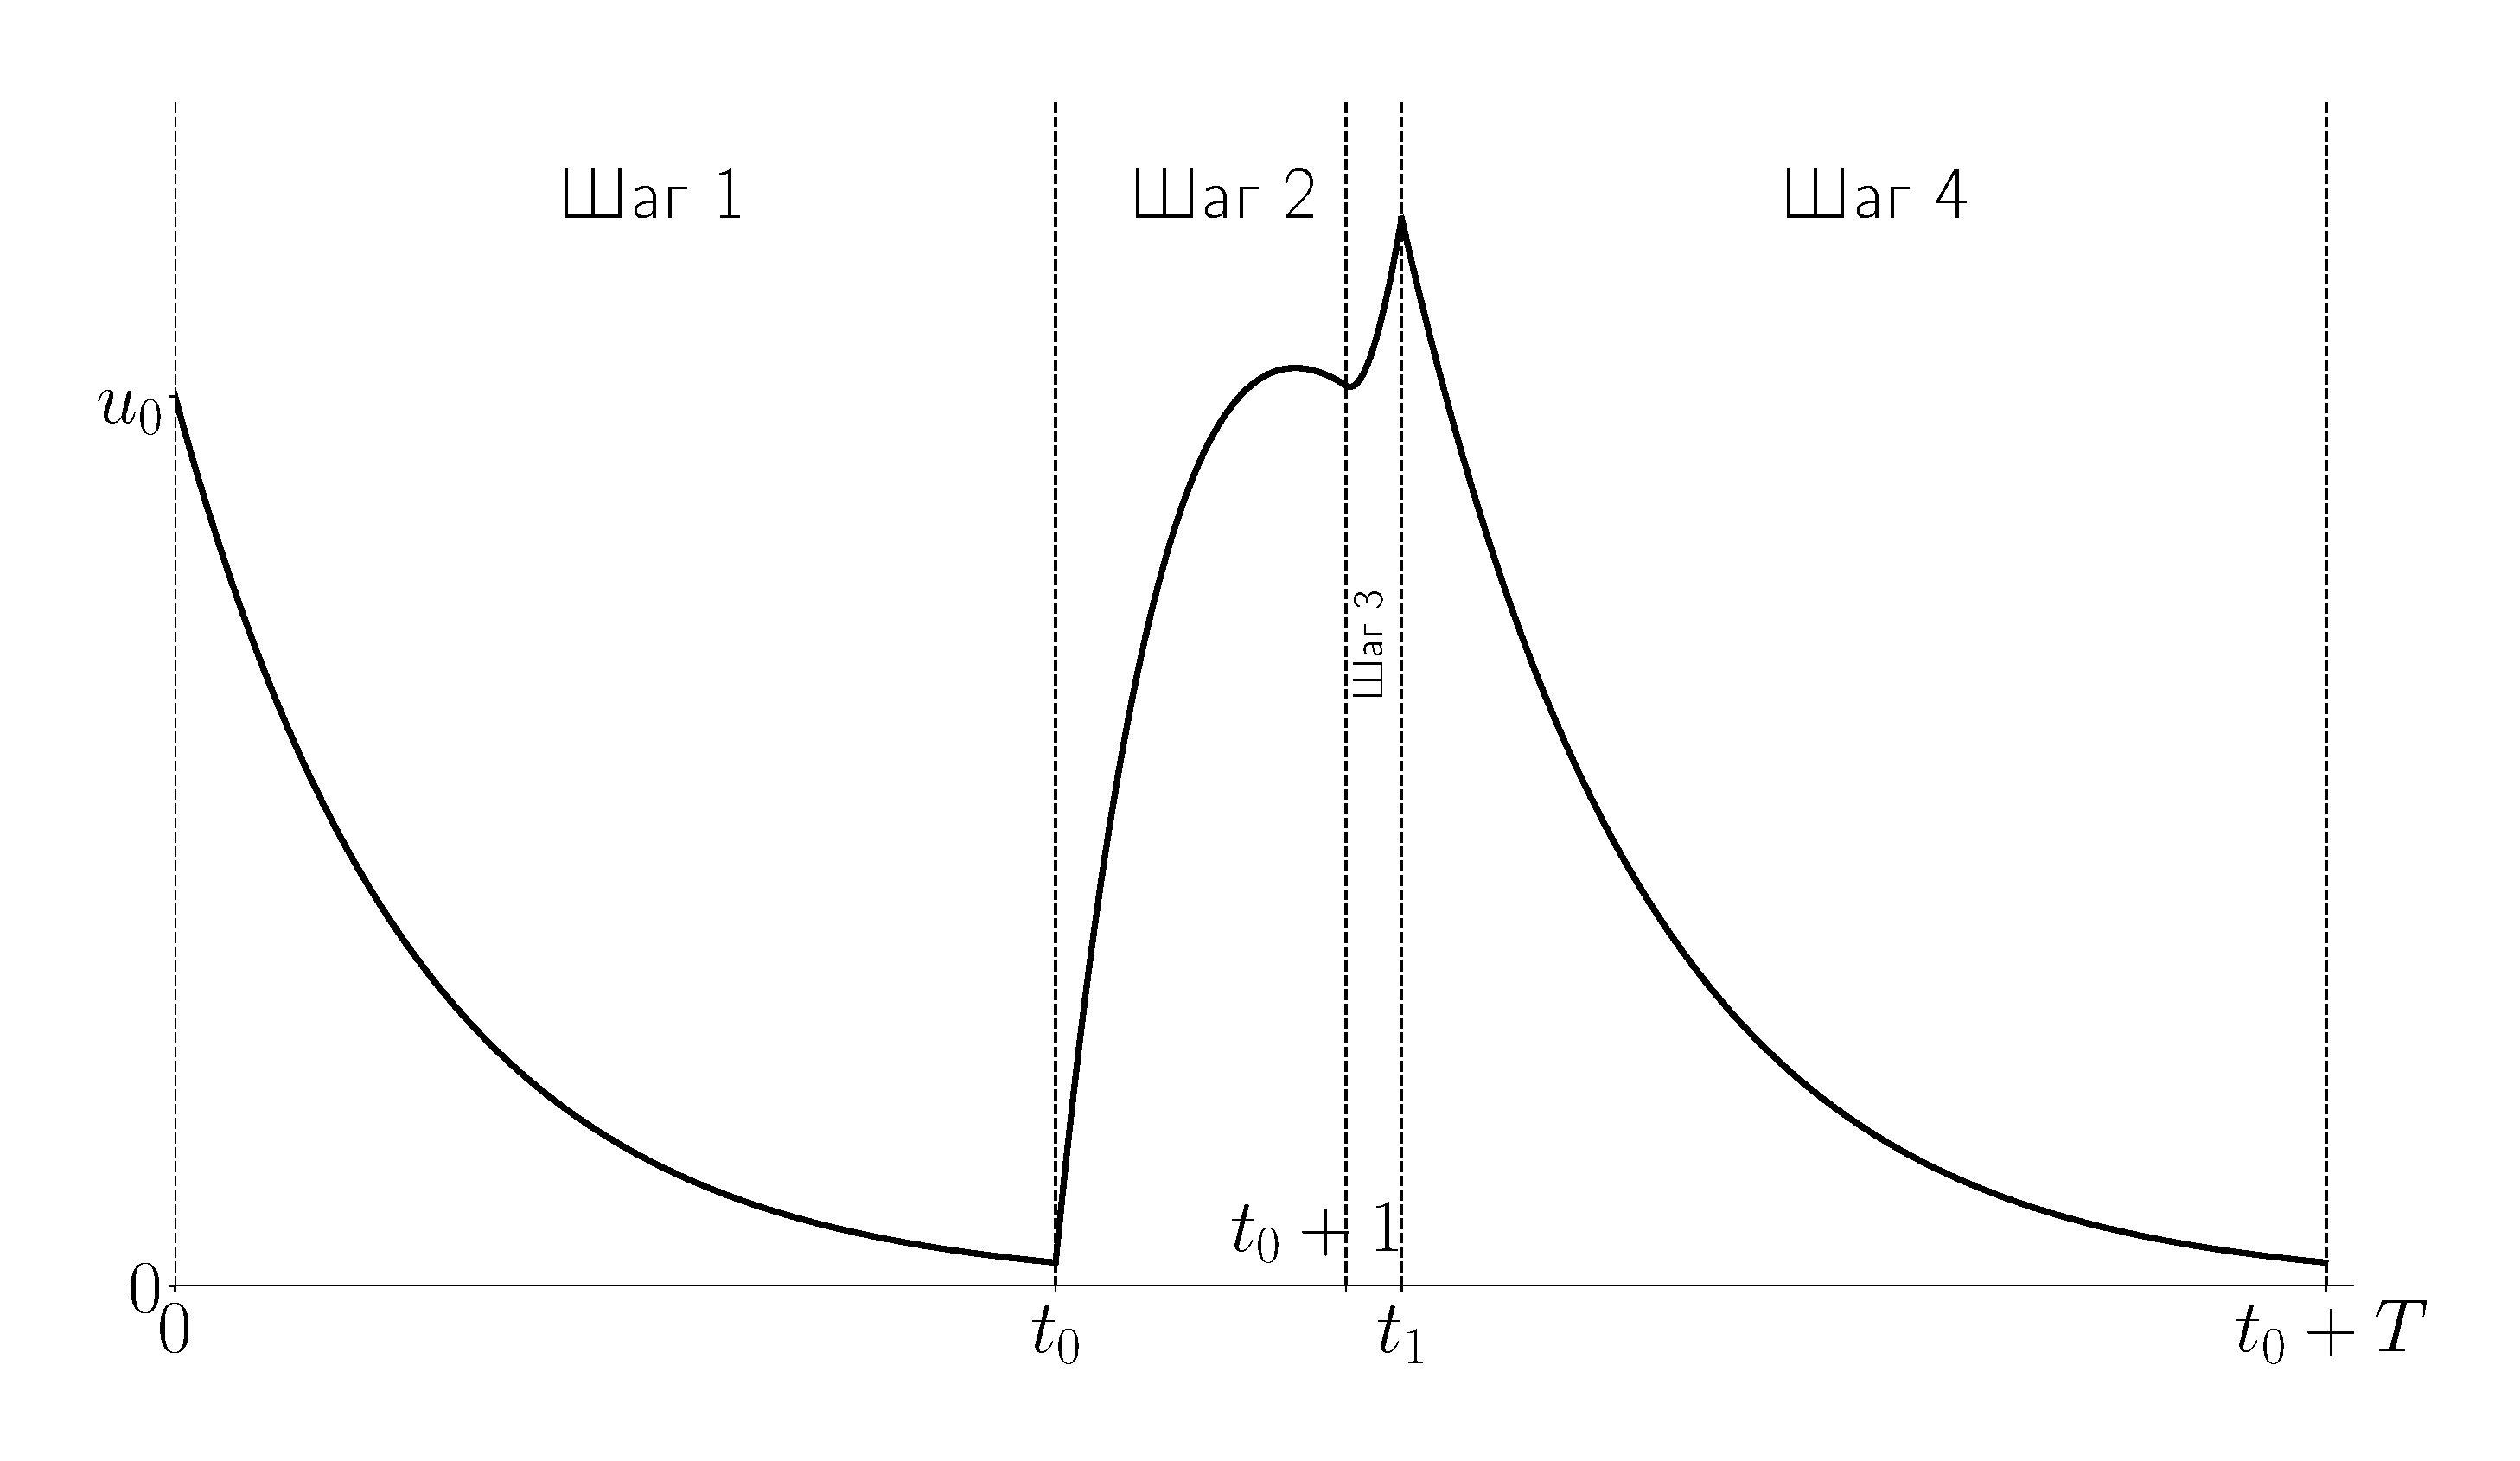
\includegraphics[width=0.7\textwidth]{u_star.eps}
	\caption{Функция $u_*(t)$, определённая на периоде $[t_0, t_0 + T]$ уравнением \eqref{eq:intro:u_star}.}
	\label{fig:intro:u_star}
\end{figure}

Для существования дискретной бегущей волны нужно проверить, что при некотором $\Delta$ период решения вспомогательного уравнения кратен $\Delta (N + 1)$, где $(N + 1)$ --- число уравнений в системе, т.е. для некоторого $p \in \mathbb{N}$ выполнено
\begin{equation}
	\label{eq:intro:period_eq}
	pT = \Delta (N + 1).
\end{equation}

Во второй главе доказывается следующая теорема.

\textbf{Теорема.} \textit{Для произвольных 
	%
	\begin{equation}
		\label{eq:intro:constraints_parameters_final}
		\beta > 0, \alpha \geq e^{\beta\left(1 + \frac{1}{e^{\beta}}\right)} - 1
	\end{equation}
	%
	найдётся $\Delta > 1$, при котором набор параметров $\alpha, \beta, \Delta$ удовлетворяет уравнению \eqref{eq:intro:period_eq} при $p = 1$ и условиям \eqref{eq:intro:cond_thm1}, \eqref{eq:intro:cond_thm2}, \eqref{eq:intro:cond_th_w>1_t_1+1}, \eqref{eq:intro:cond_hair_hair_01}, \eqref{eq:intro:cond_hair_hair_02}, \eqref{eq:intro:cond_hair_hair_1}.}

Из справедливости данной теоремы сразу следует существование решения в виде дискретной бегущей волны у системы \eqref{eq:intro:mg_full_renormed} при данных ограничениях на параметры. Численные эксперименты показывают, что решение является устойчивым; более того, результаты экспериментов позволяют предположить глобальную притягиваемость решений данного вида.

\bigskip

\pdfbookmark{Содержание третьей главы}{third}
\textbf{Содержание третьей главы.} В третьей главе рассматривается полносвязная сеть, состоящая из $N = m + n$ релейных осцилляторов Мэки--Гласса, описываемая системой \eqref{eq:intro:mg_full_renormed_delta}. Будем искать решение, описывающее режим двухкластерной синхронизации. После подстановки \eqref{eq:intro:cluster} получим вспомогательную систему \eqref{eq:intro:system_uv}.

После замен
\begin{equation}
	\label{eq:intro:tilde_change}
	\tilde{u}(t) = u(t - 1) + \delta (m - 1) u + \delta n v, \quad \tilde{v}(t) = v(t - 1) + \delta m u + \delta (n - 1) v
\end{equation}
%
и последующей экспоненциальной подстановки
\begin{equation}
	\label{eq:intro:exp_change}
	\tilde{u} = e^x, \quad \tilde{v} = e^y
\end{equation}
%
система \eqref{eq:intro:system_uv} примет вид
%
\begin{equation}
	\label{eq:intro:system_cluster_main}
	\begin{cases}
		\dot{x} = -\beta + \alpha \left(e^{x(t - 1) - x} G(x(t - 1)) + \delta (m - 1) G(x) + \delta n e^{y - x} G(y)\right),\\
		\dot{y} = -\beta + \alpha \left(e^{y(t - 1) - y} G(y(t - 1)) + \delta m e^{x - y} G(x) + \delta (n - 1) G(y)\right),
	\end{cases}
\end{equation}
где $G(x) = e^{-x} \, F(e^x)$.

Замена \eqref{eq:intro:tilde_change} корректна в смысле следующей теоремы.

\textbf{Теорема.} \textit{Пусть $(x, y)$ --- $T$-периодическое решение системы \eqref{eq:intro:system_cluster_main}. Тогда существуют $T$-периодические функции $u, v$, однозначно определяемые соотношениями \eqref{eq:intro:tilde_change}, \eqref{eq:intro:exp_change}, которые являются решением системы \eqref{eq:intro:system_uv}.}

Как и в предыдущей части диссертации, будем исследовать предельный при $\gamma \to +\infty$ объект. Подменим функцию $G$ предельной, т.~е. в уравнении \eqref{eq:intro:system_cluster_main} будем считать, что функция $G$ имеет вид 
\begin{equation}
	\label{eq:intro:relay_G_tilde}
	G(x) = \lim\limits_{\gamma \to +\infty} \dfrac{1}{1 + e^{\gamma x}} = 
	\begin{cases}
		1, & x < 0,\\
		1/2, & x = 0,\\
		0, & x > 0.
	\end{cases}
\end{equation}
%
В этом случае правая часть релейной системы \eqref{eq:intro:system_cluster_main} терпит разрыв при $x = 0$ и при $y = 0$. Анализ системы показывает, что её решение при достижении одной из прямых разрыва может продолжаться только вдоль этой прямой (трансверсальное пересечение прямой разрыва оказывается невозможным). В связи с этим находится обобщённое решение системы: положим, что при $x \neq 0$ функция $G$ описывается формулой \eqref{eq:intro:relay_G_tilde}, а в случае $x = 0$ принимает то значение из промежутка $(0, 1)$, при котором решение $(x, y)$ продолжается вдоль прямой $x = 0$; аналогично определяется движение по прямой $y = 0$. В такой постановке данный метод соответствует методу эквивалентного управления \cite{Utkin1981}. %, однако в силу специфики данной системы, такое доопределение оказывается эквивалентным другим вариантам обобщения понятия решения системы дифференциальных уравнений, приведённым в \cite{Filippov1988}.


Определим на множестве $[-1, 0]$ семейство пар начальных функций. Фиксируем $x_0 > y_0 > 0$.
\begin{equation}
	\label{eq:intro:initial_set}
	S = \left\{\phi, \psi \in C[-1, 0] \,|\, \phi(t) > 0, \psi(t) > 0, x_0 = \phi(0), y_0 = \psi(0)\right\}.
\end{equation}

Доказана следующая теорема.

\bigskip

\textbf{Теорема.}
\textit{Пусть}
%
\begin{equation}
	\label{eq:intro:constraint_1}
	x_0 - y_0 < \ln \dfrac{e^{2\beta}(n - \delta(n - 1)) - ne^{\beta} + \delta n(n - 1)}{\delta (n - 1)^2},
\end{equation}
\begin{equation}
	\label{eq:intro:constraint_2}
	\beta < \alpha \delta (m - 1), \quad \beta < \alpha \delta (n - 1),
\end{equation}
\small
\begin{equation}
	\label{eq:intro:constraint_3}
	e^{\beta} \cdot \dfrac{n - \delta(n - 1)}{\delta (n - 1)^2} > \dfrac{1}{n - 1} + \dfrac{1}{\delta(m - 1)}, \quad
	e^{\beta} \cdot \dfrac{m - \delta(m - 1)}{\delta (m - 1)^2} > \dfrac{1}{\delta(n - 1)} + \dfrac{1}{m - 1}.
\end{equation}
\normalsize

\textit{При ограничениях \eqref{eq:intro:constraint_1}, \eqref{eq:intro:constraint_2}, \eqref{eq:intro:constraint_3}  и произвольных начальных функциях из множества \eqref{eq:intro:initial_set} релейная система \eqref{eq:intro:system_cluster_main} имеет обобщённое решение, описываемое формулами}
%
\small
\begin{equation}
	\label{eq:intro:step1_solution}
	\begin{cases}
		x = x_0 - \beta t,\\
		y = y_0 - \beta t
	\end{cases}
	\text{при } t \in [0, t_0], \text{ где } t_0 = \dfrac{y_0}{\beta};
\end{equation}
%
\begin{equation}
	\label{eq:intro:step2_solution}
	\begin{cases}
		x = x_0 - \beta t + \ln\left(1 + \frac{n}{n - 1} e^{-x_0 + \beta t_0}  (e^{\beta  (t - t_0)} - 1)\right),\\
		y = 0
	\end{cases}
	\text{при } t \in [t_0, t_0 + 1];
\end{equation}
%
\begin{multline}
	\label{eq:intro:step3_solution}
	\begin{cases}
		x = -\beta t + \ln\left(\exp(x(t_{2i} + 1) + \beta (t_{2i} + 1)) + \frac{n (\delta(n - 1) - 1)}{\delta (n - 1)^2} (e^{\beta t} - \exp(\beta (t_{2i} + 1)))\right)
		,\\
		y = 0
	\end{cases}\\
	\text{при } t \in [t_{2i} + 1, t_{2i + 1}];
\end{multline}
%
\begin{multline}
	\label{eq:intro:step4_solution}
	\begin{cases}
		x = 0,\\
		y = -\beta t + \ln\left(\exp(\beta t_{2i + 1}) + \left(\frac{1}{\delta(n - 1)} + \frac{m}{m - 1}\right) (e^{\beta t} - \exp(\beta t_{2i + 1}))\right)
	\end{cases}\\
	\text{при } t \in [t_{2i + 1}, t_{2i} + 2];
\end{multline}
%
\begin{multline}
	\label{eq:intro:step5_solution}
	\begin{cases}
		x = 0,\\
		y = -\beta t + \ln\bigg(\exp(y(t_{2i} + 2) + \beta (t_{2i} + 2)) + \bigg(\frac{\delta(n - 1) - 1}{\delta^2 (n - 1)^2} + \frac{m}{m - 1}\bigg) (e^{\beta t} - \exp(\beta (t_{2i} + 2)))\bigg)
	\end{cases}\\
	\text{при } t \in [t_{2i} + 2, t_{2i + 1} + 1];
\end{multline}
%
\begin{multline}
	\label{eq:intro:step6_solution}
	\begin{cases}
		x = 0,\\
		y = -\beta t + \ln\left(\exp(y(t_{2i + 1} + 1) + \beta(t_{2i + 1} + 1)) + \frac{m (\delta (m - 1) - 1)}{\delta (m - 1)^2} (e^{\beta t} - \exp(\beta (t_{2i + 1} + 1))) \right)
	\end{cases}\\
	\text{при } t \in [t_{2i + 1} + 1, t_{2i + 2}];
\end{multline}
%
\begin{multline}
	\label{eq:intro:step7_solution}
	\begin{cases}
		x = -\beta t + \ln\left(\exp(\beta t_{2i + 2}) + \left(\frac{1}{\delta(m - 1)} + \frac{n}{n - 1}\right) (e^{\beta t} - \exp(\beta t_{2i + 2}))\right),\\
		y = 0
	\end{cases}\\
	\text{при } t \in [t_{2i + 2}, t_{2i + 1} + 2];
\end{multline}
%
\begin{multline}
	\label{eq:intro:step8_solution}
	\begin{cases}
		x = -\beta t + \ln\left(\exp(x(t_{2i + 1} + 2) + \beta (t_{2i + 1} + 2)) + \left(\frac{\delta(m - 1) - 1}{\delta^2 (m - 1)^2} + \frac{n}{n - 1}\right) (e^{\beta t} - \exp(\beta (t_{2i + 1} + 2)))\right),\\
		y = 0
	\end{cases}\\
	\text{при } t \in [t_{2i + 1} + 2, t_{2i + 2} + 1];
\end{multline}
%
\begin{multline}
	\label{eq:intro:step9_solution}
	\begin{cases}
		x = -\beta t + \ln\left(\exp(y(t_{2i + 2} + 1) + \beta(t_{2i + 2} + 1)) + \frac{n (\delta(n - 1) - 1)}{\delta (n - 1)^2} (e^{\beta t} - \exp(\beta (t_{2i + 2} + 1))) \right),\\
		y = 0
	\end{cases}\\
	\text{при } t \in [t_{2i + 2} + 1, t_{2i + 3}].
\end{multline}
\normalsize
%	
\textit{Здесь $i \geqslant 0$ --- целое число. Каждый момент времени $t_{2i + 1}$ определяется как корень уравнения $x = 0$, где функция $x(t)$ задаётся уравнением \eqref{eq:intro:step3_solution}. Каждый момент времени $t_{2i + 2}$ определяется как корень уравнения $y(t) = 0$, где функция $y(t)$ определяется из системы \eqref{eq:intro:step6_solution}. Для всех $i \geqslant 0$ верно, что $t_{i + 1} \in (t_i + 1, t_i + 2)$.}


\begin{figure}[!ht]
	\centering
	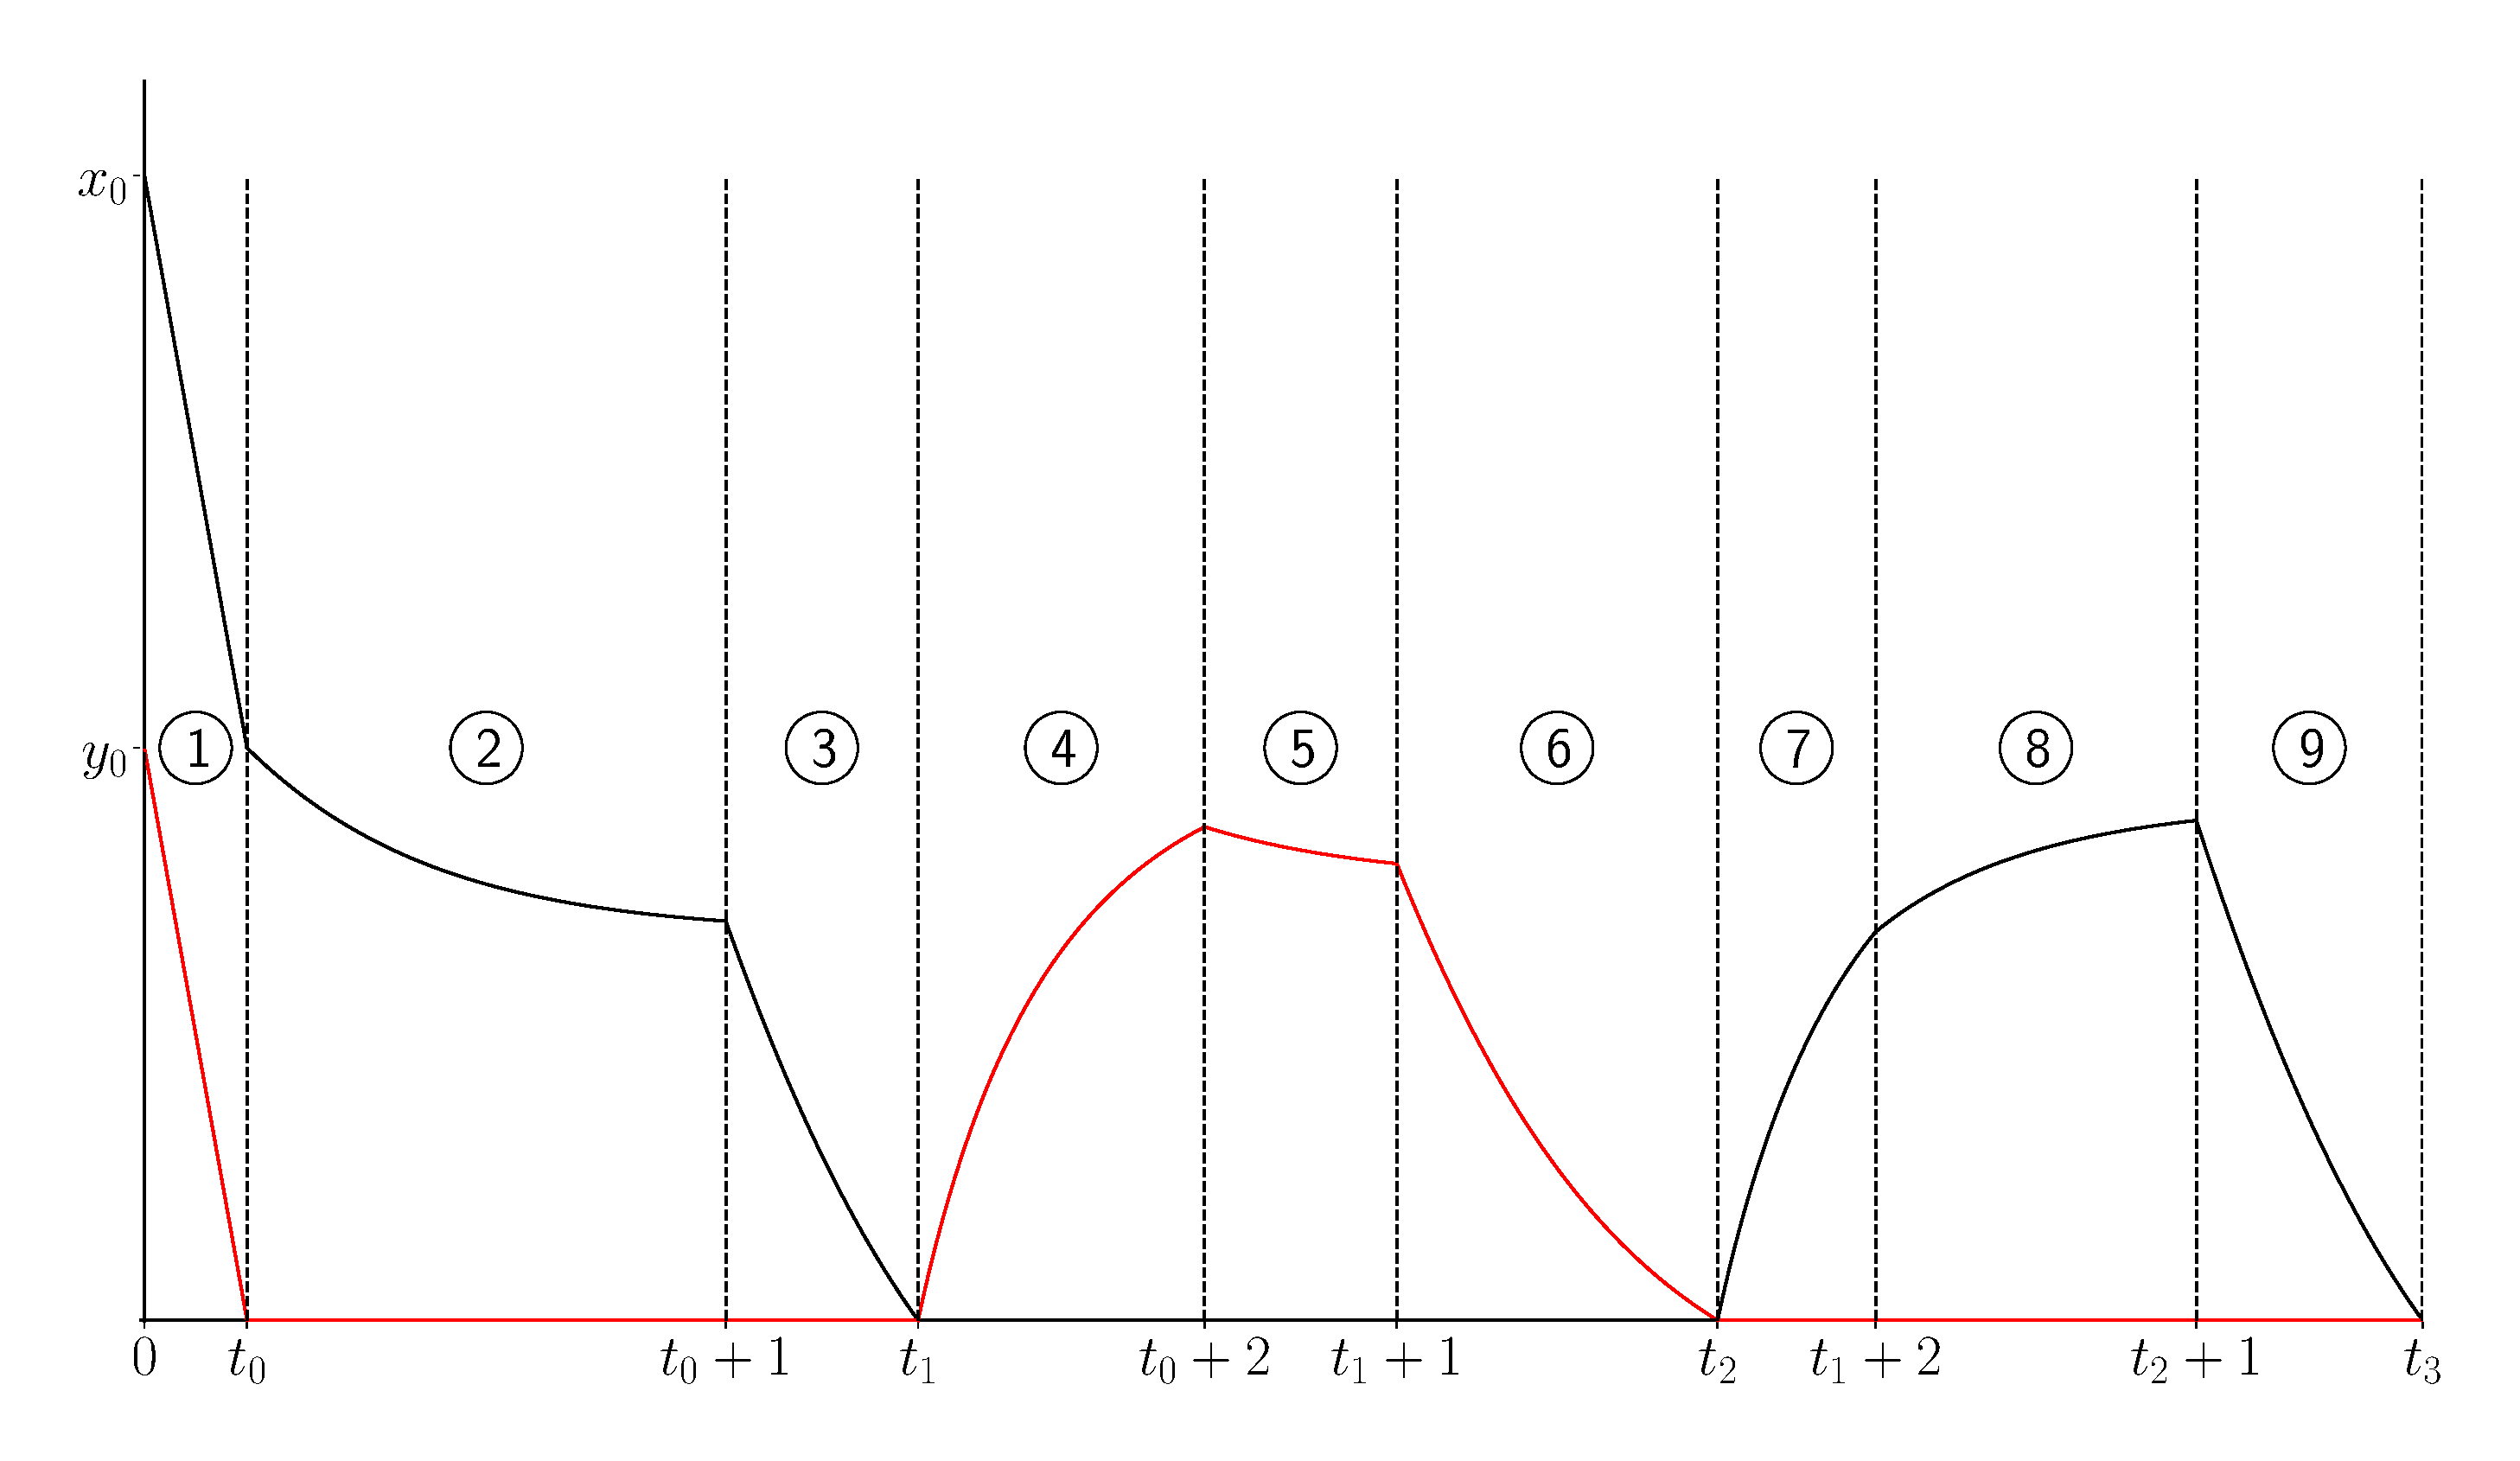
\includegraphics[width=\textwidth]{cluster_step_by_step.eps}
	\caption{Обобщённое решение релейной системы \eqref{eq:intro:system_cluster_main}, построенное методом шагов. Чёрная линия --- компонента решения $x$, красная линия --- компонента решения $y$. Числа в кругах --- номер шага построения.}
	\label{fig:intro:cluster_step_by_step}
\end{figure}

Основным результатом третьей главы является следующая теорема.

\textbf{Теорема.} \textit{При ограничениях \eqref{eq:intro:constraint_1}, \eqref{eq:intro:constraint_2}, \eqref{eq:intro:constraint_3} релейная система \eqref{eq:intro:system_cluster_main} имеет периодическое решение, описываемое на периоде $[t_1, t_3]$ формулами \eqref{eq:intro:step4_solution} -- \eqref{eq:intro:step9_solution}.}

\FloatBarrier
\pdfbookmark{Заключение}{conclusion}                                  % Закладка pdf
В \textbf{заключении} приведены основные результаты работы, которые заключаются в следующем:
%% Согласно ГОСТ Р 7.0.11-2011:
%% 5.3.3 В заключении диссертации излагают итоги выполненного исследования, рекомендации, перспективы дальнейшей разработки темы.
%% 9.2.3 В заключении автореферата диссертации излагают итоги данного исследования, рекомендации и перспективы дальнейшей разработки темы.

\begin{enumerate}
  \item Получены асимптотические формулы периодического решения уравнения Мэки--Гласса для достаточно больших значений коэффициента нелинейности. Показано, что из асимптотических соотношений следует сходимость решения уравнения Мэки--Гласса к решению соответствующего предельного релейного уравнения.
  \item Сформулированы и доказаны достаточные условия существования периодических режимов (а) в виде дискретной бегущей волны, (б) двухкластерной синхронизации в полносвязной цепи релейных генераторов Мэки--Гласса в виде ограничения на параметры соответствующей системы дифференциальных уравнений с запаздыванием. 
  \item Проведено численное моделирование, демонстрирующее устойчивость соответствующих режимов.
\end{enumerate}


\pdfbookmark{Литература}{bibliography}                               % Закладка pdf

\ifdefmacro{\microtypesetup}{\microtypesetup{protrusion=false}}{} % не рекомендуется применять пакет микротипографики к автоматически генерируемому списку литературы
\urlstyle{rm}                               % ссылки URL обычным шрифтом
\ifnumequal{\value{bibliosel}}{0}{% Встроенная реализация с загрузкой файла через движок bibtex8
    \renewcommand{\bibname}{\large \bibtitleauthor}
    \nocite{*}
    \insertbiblioauthor           % Подключаем Bib-базы
    %\insertbiblioexternal   % !!! bibtex не умеет работать с несколькими библиографиями !!!
}{% Реализация пакетом biblatex через движок biber
    % Цитирования.
    %  * Порядок перечисления определяет порядок в библиографии (только внутри подраздела, если `\insertbiblioauthorgrouped`).
    %  * Если не соблюдать порядок "как для \printbibliography", нумерация в `\insertbiblioauthor` будет кривой.
    %  * Если цитировать каждый источник отдельной командой --- найти некоторые ошибки будет проще.
    %
    %% authorvak
    \nocite{vakbib1}%
    \nocite{vakbib2}%
    %
    %% authorwos
    \nocite{wosbib1}%
    %
    %% authorscopus
    \nocite{scbib1}%
    %
    %% authorpathent
    \nocite{patbib1}%
    %
    %% authorprogram
    \nocite{progbib1}%
    %
    %% authorconf
    \nocite{confbib1}%
    \nocite{confbib2}%
    %
    %% authorother
    \nocite{bib1}%
    \nocite{bib2}%

    \ifnumgreater{\value{usefootcite}}{0}{
        \begin{refcontext}[labelprefix={}]
            \ifnum \value{bibgrouped}>0
                \insertbiblioauthorgrouped    % Вывод всех работ автора, сгруппированных по источникам
            \else
                \insertbiblioauthor      % Вывод всех работ автора
            \fi
        \end{refcontext}
    }{
        \ifnum \totvalue{citeexternal}>0
            \begin{refcontext}[labelprefix=A]
                \ifnum \value{bibgrouped}>0
                    \insertbiblioauthorgrouped    % Вывод всех работ автора, сгруппированных по источникам
                \else
                    \insertbiblioauthor      % Вывод всех работ автора
                \fi
            \end{refcontext}
        \else
            \ifnum \value{bibgrouped}>0
                \insertbiblioauthorgrouped    % Вывод всех работ автора, сгруппированных по источникам
            \else
                \insertbiblioauthor      % Вывод всех работ автора
            \fi
        \fi
        %  \insertbiblioauthorimportant  % Вывод наиболее значимых работ автора (определяется в файле characteristic во второй section)
        \begin{refcontext}[labelprefix={}]
            \insertbiblioexternal            % Вывод списка литературы, на которую ссылались в тексте автореферата
        \end{refcontext}
        % Невидимый библиографический список для подсчёта количества внешних публикаций
        % Используется, чтобы убрать приставку "А" у работ автора, если в автореферате нет
        % цитирований внешних источников.
        \printbibliography[heading=nobibheading, section=0, env=countexternal, keyword=biblioexternal, resetnumbers=true]%
    }
}
\ifdefmacro{\microtypesetup}{\microtypesetup{protrusion=true}}{}
\urlstyle{tt}                               % возвращаем установки шрифта ссылок URL
